\documentclass[12pt]{article}
\usepackage[margin=1in]{geometry}
\usepackage{newtxtext,newtxmath}
\usepackage{amsmath,booktabs,graphicx,microtype,setspace,caption}
\usepackage[round,semicolon]{natbib}
\usepackage[colorlinks=true,citecolor=blue,linkcolor=black,urlcolor=blue]{hyperref}
\graphicspath{{figs/}}
\captionsetup{font=small,labelfont=bf,justification=justified}
\newcommand{\dR}{\Delta R^2}
\onehalfspacing

\begin{document}

%---------------- Title page ----------------
\begin{titlepage}
\begin{center}
{\Large\bfseries Hidden States Beat Summary Statistics:\\[2pt]
Extracting Intraday Volatility Information from a\\[2pt]
Frozen Time-Series Foundation Model\footnote{We thank seminar participants for
helpful comments. All remaining errors are our own. Code and complete
experimental logs are available from the author.}}\\[20pt]

% 作者署名从仓库中移除(用户 2026-09-17 指示: 个人信息不入仓)。
% 投稿/编译正式版时, 取消下一行注释并填入署名, 或维护未跟踪的 paper/author.local.tex。
% {\large <AUTHOR>\footnote{Contact: <EMAIL>.}}\\[2pt]
{\large Anonymous}\\[2pt]
%~\\[16pt]
{\today}
\end{center}

\vspace{10pt}
\begin{center}{\bfseries Abstract}\end{center}
\begin{quote}
\singlespacing\small
\noindent
Time-series foundation models (TSFMs) are commonly evaluated in finance through
scalar summaries of their predictive distribution---negative log-likelihood or
predictive entropy---and on that basis have been judged nearly useless for index
risk management. We show that this verdict is an artifact of the
\emph{extraction interface}, not the model. Feeding the full 512-dimensional
hidden state of a frozen, zero-shot K-line foundation model into a
35K-parameter gated corrector on top of a strong HAR-type baseline raises the
out-of-sample gain in one-hour-ahead index volatility forecasts by an order of
magnitude: on a pre-registered, one-shot holdout year,
$\dR = +0.095 \pm 0.004$ across 100 seeds (none negative), with QLIKE
improvements of 17--21\% (Diebold--Mariano $t$ up to 7.6, Clark--West $t$ up to
16.9). The hidden state subsumes a 500-constituent cross-sectional breadth
signal and, on 133 holdout days of five-minute index-option order-book data,
the option market's own implied volatility; it is essentially 100\% novel
relative to known volatility variables, and helps most exactly when the
baseline is weakest. Its incremental value traces an inverted-U in the forecast
horizon that peaks at one hour, a curve that predicts both where the forecast
can be monetized and where it cannot. A same-input scratch
Transformer matches the frozen pipeline only with the full nine-year training
sample; with half the data the frozen representation retains 77\% of its gain
versus 34\% for the scratch model. The economic value of pretraining is thus
sample efficiency in the practically relevant data regime, not asymptotic
accuracy. Direction remains unpredictable throughout and the information
horizon is strictly intraday. A volatility-targeted overlay on CSI~500/1000
index futures under realistic Chinese transaction costs converts the forecast
upgrade into 460--970 basis points per year relative to an identical overlay
driven by the baseline forecast, although strategy-level bootstrap intervals
still include zero---an explicit illustration of the gap between forecast
significance and portfolio significance.
\end{quote}

\vspace{8pt}
\noindent\textbf{JEL codes:} C45, C53, C58, G17.\\
\textbf{Keywords:} time-series foundation models, transfer learning, realized
volatility, volatility-managed portfolios, index futures.
\end{titlepage}

%---------------- 1 Introduction ----------------
\section{Introduction}
Pretrained foundation models for time series promise transferable
representations of temporal structure \citep{das2024timesfm,ansari2024chronos,
shi2025kronos}, yet their record in quantitative finance is mixed. A common
evaluation pattern treats the TSFM as a probabilistic forecaster and extracts
one or two scalars---the negative log-likelihood (NLL) of realized outcomes, or
the entropy of the one-step predictive distribution---as ``model-based'' risk
factors. In our own prior work, ten successive evaluations of such scalars on
Chinese index data produced economically null results and led the program to be
shut down.

This paper documents a precise reversal of that verdict. Holding the model, the
data, the baseline, and the evaluation protocol fixed, we change only the
\emph{extraction interface}: instead of two scalars we use the full
512-dimensional final hidden state of the frozen decoder, mapped through a
small gated linear corrector in the spirit of \citet{dewage2026hybrid}. The
increment to one-hour-ahead volatility forecasts rises by an order of
magnitude and survives a battery of falsification tests: a pre-registered
one-shot holdout year, one hundred re-trainings from independent seeds, placebo
shuffling of the hidden states, nested-model \citet{clark2007cw} tests, and a
model confidence set \citep{hansen2011mcs} that eliminates every specification
without hidden states.

Three findings characterize \emph{what} the representation knows. First,
second moments only: direction is unpredictable in every configuration
($R^2 \approx 0$), symmetric tail volatility inherits the full gain, while
signed tail objectives (value-at-risk, crash probability) gain little. Second,
the incremental value traces an inverted-U in the forecast horizon, rising from
$+0.013$ at five minutes to $+0.084$ at one hour and collapsing to $+0.009$ for
next-day realized variance: the representation encodes a regime at a
characteristic timescale of about an hour. Third, the
single-index hidden state \emph{subsumes} cross-sectional breadth:
conditioning on it drives the incremental value of a breadth-entropy signal
built from all 500 index constituents to zero, while the converse does not
hold.

Two further experiments discipline the interpretation. A scratch Transformer
trained end-to-end on the identical input window matches the frozen pipeline at
full sample size (only the test segment retains a gap), but falls far behind
when training data is restricted to realistic spans: with 4.5 years of data
the frozen representation attains 77\% of its full-sample holdout gain versus
34\% for the scratch model, and with half a year both fail. The premium of
pretraining is therefore \emph{sample efficiency and cross-regime stability},
not an asymptotically unreachable representation. Second, transfer tests show
that the representation is universal across indices while the corrector is
family-specific: a corrector trained on two broad-cap indices transfers at
full strength to a third within the family, but zero-shot transfer to style
indices retains only a small fraction of the gain, which local re-fitting of
the 35K-parameter corrector restores.

Finally, we take the forecast to the futures market with production-grade
accounting: official dominant-contract mapping lagged one day, within-contract
returns including overnight gaps, roll costs, and the asymmetric Chinese fee
schedule under which intraday close-outs cost roughly seven times more than
opens. A no-trade band is what keeps the overlay alive under these costs.
The forecast upgrade is worth 460--970 basis points per year against an
identical overlay driven by the baseline forecast (six of six index-segment
cells positive; best cell $t=2.3$), yet strategy-level bootstrap intervals
still include zero: forecast significance does not automatically become
portfolio significance, and the deployment we endorse is an exposure-management
overlay for accounts that already hold a net long index-futures position.

\medskip
\noindent\textbf{Related literature.} Our paper connects three strands.
The first is the emerging literature on time-series foundation models:
TimesFM \citep{das2024timesfm}, Chronos \citep{ansari2024chronos}, and the
K-line-specialized Kronos \citep{shi2025kronos} pretrain autoregressive
forecasters on large corpora. \citet{dewage2026hybrid} document that frozen
TSFMs are weak in high-frequency finance unless paired with lightweight
neural-classical correctors; our corrector follows their gated architecture,
but our ablations reverse their attribution---with a strong baseline that
already absorbs seasonality and multi-scale realized volatility, tree-based
residual learners add nothing after the gated corrector. We also show the
phenomenon is not model-specific: a univariate Chronos encoder carries real,
though three times weaker, volatility information on the same task. The second
strand is volatility forecasting. Our baseline follows the HAR tradition of
\citet{corsi2009har} with multi-scale realized components and intraday
seasonality dummies; HARQ-type corrections \citep{bollerslev2016harq} add
nothing at the daily horizon in our data. Losses and tests follow
\citet{patton2011volatility}, \citet{diebold1995dm}, \citet{clark2007cw}, and
\citet{hansen2011mcs}. The third strand is volatility-managed portfolios
\citep{moreira2017volmanaged}: our overlay is an intraday, forecast-upgraded
variant, and we show that the scaling exponent ($1/\sigma$ versus
$1/\sigma^2$) is a regime bet orthogonal to forecast quality.

The remainder of the paper proceeds as follows. Section~\ref{sec:data}
describes the data. Section~\ref{sec:method} presents the frozen
representation and the corrector. Section~\ref{sec:baseline} contains the
baseline forecasting results and their statistical validation.
Section~\ref{sec:nature} characterizes the nature of the extracted
information. Section~\ref{sec:pretraining} asks whether pretraining is
necessary. Section~\ref{sec:econ} evaluates the futures overlay under
realistic costs. Section~\ref{sec:robust} summarizes robustness, and
Section~\ref{sec:conclusion} concludes.

%---------------- 2 Data ----------------
\section{Data}\label{sec:data}
\textbf{Indices.} We use 5-minute OHLCV-plus-amount bars for the CSI~300,
CSI~500, and CSI~1000 indices, aggregated from an authoritative one-minute
database, covering January 2014 through August 2026 (3{,}068 trading days, 48
bars per day, no missing bars). Decision points are bars 0--35 of each day, so
that the forecast window remains within the trading session, yielding
324{,}157 index-bar observations of which 315{,}045 survive feature filters.
Transfer experiments additionally use the SSE~50, ChiNext, and STAR~50
indices from the same source.

\textbf{Futures.} The economic application uses IC (CSI~500) and IM
(CSI~1000) index futures. We construct dominant-contract series from the
official dominant map lagged by one day (so the contract held on day $t$ is
known at the close of $t-1$), compute within-contract 5-minute returns plus
same-contract overnight returns, and account for rolls explicitly (135 rolls
for IC over 2015--2026).

\textbf{Sample splits.} The training sample ends 2023-04-27; the validation
sample (used for early stopping and \emph{all} selection) ends 2024-06-07; the
test sample (reporting only) ends 2025-07-17; and the holdout sample covers
2025-07-18 through 2026-08-14 (262 days) and is \emph{pre-registered and
opened exactly once} after all modeling decisions were fixed.

\textbf{Target.} The forecast objective is
$y_t = \log\big(\tfrac1H \sum_{i=1}^{H} |r_{t+i}|\big)$ with $H=12$ (one hour)
or $H=24$ (two hours), where $r$ denotes 5-minute log returns and overnight
bars are excluded. A directional control target $\sum_i r_{t+i}$ is carried
through every experiment.

%---------------- 3 Methodology ----------------
\section{Methodology}\label{sec:method}
\subsection{Frozen representation}
Each decision point feeds the frozen Kronos-small decoder a window of $L=128$
bars, z-scored \emph{within the window} and clipped at $\pm5$:
\begin{equation}
\tilde{x}_{t-i} \;=\; \mathrm{clip}\!\big((x_{t-i}-\mu_W)/(\sigma_W+\varepsilon),\,-5,\,5\big),
\qquad i = 0,\dots,L-1 .
\end{equation}
Window-local normalization forces one independent forward pass per decision
point; sliding-window reuse would leak future bars into the normalizer. From
the forward pass we keep the final hidden state
$\mathbf{h}_t = \mathrm{ctx}[\,:, L{-}1, :\,] \in \mathbb{R}^{512}$ and, as the
scalar-interface control, the NLL and the one-step predictive entropy. The
model is never fine-tuned.

\subsection{Baseline and corrector}
The baseline is a deliberately strong ridge regression,
\begin{equation}
\hat{y}^{0} = \mathbf{x}_b^{\top}\hat\beta, \qquad
\hat\beta = (X_{\mathrm{tr}}^\top X_{\mathrm{tr}} + \lambda I)^{-1}
X_{\mathrm{tr}}^\top \mathbf{y}_{\mathrm{tr}},
\end{equation}
where $\mathbf{x}_b$ stacks log realized-volatility components at one-hour,
four-hour and five-day scales, the current absolute return, intraday-bar
dummies, and index dummies. The corrector is a low-rank gated linear map on
$\mathbf{x} = [\mathbf{x}_b;\,\mathrm{nll};\,\mathrm{ent};\,\mathbf{h}]
\in \mathbb{R}^{556}$:
\begin{equation}
\Delta\hat{y} = \mathbf{w}_o^{\top}\big(\sigma(W_g\mathbf{x}) \odot
W_r\mathbf{x}\big) + b, \qquad
\hat{y}^{M2} = \hat{y}^{0} + \Delta\hat{y},
\end{equation}
with rank 32 (about 35K parameters), trained on baseline residuals with Adam
and validation early stopping. Coefficients are frozen at the training
boundary; an annual walk-forward refit changes out-of-sample $R^2$ by at most
$\pm0.005$ over three years.

\subsection{Evaluation metrics}
Beyond incremental $R^2$, we track four statistics. The \emph{daily rank IC}
of the incremental signal is the within-day Spearman correlation between the
corrector's increment and the baseline residual,
\begin{equation}
\mathrm{IC}_d = \rho^{S}\!\big(\Delta\hat{y}_t,\; y_t - \hat{y}^{0}_t\big)_{t \in d},
\qquad
\mathrm{IR} = \frac{\overline{\mathrm{IC}}}{\mathrm{sd}(\mathrm{IC})},
\qquad t = \mathrm{IR}\sqrt{n_d}.
\end{equation}
Forecast losses use QLIKE on variance forecasts with a train-sample
multiplicative bias correction \citep{patton2011volatility},
\begin{equation}
\mathrm{QLIKE}(F_t, RV_t) = \frac{RV_t}{F_t} - \log\frac{RV_t}{F_t} - 1,
\qquad F_t = \big(c\,e^{\hat{y}_t}\big)^2 ,\;
c = \exp\!\big(\overline{y-\hat{y}}\big)_{\mathrm{tr}}.
\end{equation}
Loss comparisons aggregate to daily means and use the \citet{diebold1995dm}
statistic with a Newey--West variance (lag 5). Because the baseline is nested
in the corrected model, we also report the \citet{clark2007cw} adjusted
differential
\begin{equation}
f_t = e_{0,t}^2 - e_{1,t}^2 + \big(\hat{y}^{0}_t - \hat{y}^{M2}_t\big)^2 ,
\end{equation}
whose daily mean is tested in the same way. Model comparisons across the full
specification set use the model confidence set of \citet{hansen2011mcs} on
daily QLIKE losses with a stationary block bootstrap.

%---------------- 4 Baseline results ----------------
\section{Baseline Forecasting Results}\label{sec:baseline}
Table~\ref{tab:main} and Figure~\ref{fig:extraction} contain the headline
result. The scalar interface reproduces the historical null
($+0.003$--$0.005$); the full hidden state through the gated corrector
delivers $\dR = +0.065/+0.042/+0.096$ on validation/test/holdout, with a
100-seed holdout mean of $+0.095\pm0.004$ (minimum seed $+0.084$, none
negative). LGBM applied to the same features confirms the attribution:
without the hidden state it recovers only $+0.013$--$0.019$; with it,
$+0.035$--$0.079$. A tree stacked after the gated corrector adds at most
$0.002$: with a strong baseline, the classical residual stage of
\citet{dewage2026hybrid} has nothing left to learn.

\begin{table}[t]
\centering\small
\caption{\textbf{One-hour-ahead volatility: incremental $R^2$ over the strong
baseline.} The dependent variable is log mean absolute 5-minute return over
the next hour. The baseline is a ridge regression on multi-scale realized
volatility, the current absolute return, intraday-bar dummies, and index
dummies, with coefficients frozen at the training boundary. The holdout
(2025-07-18 to 2026-08-14) is pre-registered and opened once. The daily IC is
the within-day Spearman rank correlation between the incremental prediction
and the baseline residual; the daily IR is its mean over its standard deviation (a
signal-strength ratio independent of sample length), and $t$ multiplies the IR
by $\sqrt{n_d}$.}
\label{tab:main}
\vspace{6pt}
\begin{tabular}{lcccc}
\toprule
Model & Validation & Test & Holdout & Holdout daily IC (IR; $t$) \\
\midrule
Scalars (NLL + entropy) & $+0.003$ & $+0.005$ & --- & --- \\
Ridge + hidden state & $+0.054$ & $+0.034$ & $+0.084$ & --- \\
LGBM residual (no hidden) & $+0.018$ & $+0.013$ & $+0.019$ & $+0.098$ (0.37; 5.9) \\
LGBM residual (+ hidden) & $+0.055$ & $+0.035$ & $+0.079$ & $+0.292$ (1.04; 16.9) \\
GatedLinear (+ hidden) & $\mathbf{+0.065}$ & $\mathbf{+0.042}$ & $\mathbf{+0.096}$ & $\mathbf{+0.377}$ (\textbf{1.41}; 22.9) \\
\bottomrule
\end{tabular}
\end{table}


\begin{figure}[t]
\centering
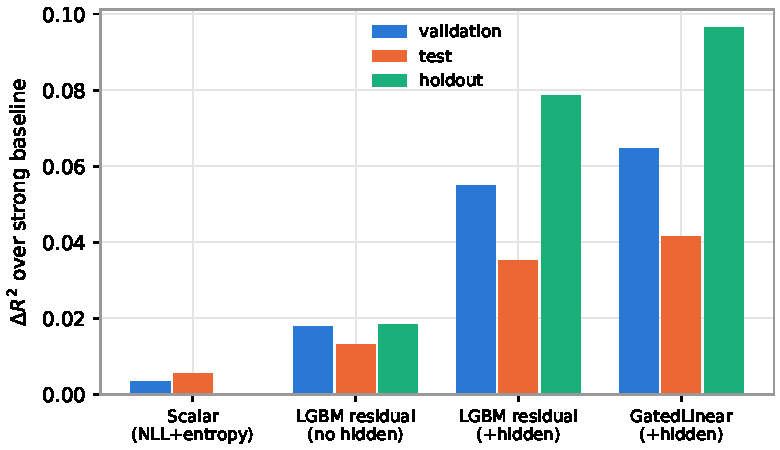
\includegraphics[width=.8\linewidth]{fig_extraction}
\caption{\textbf{The extraction interface is the bottleneck.} Incremental
$R^2$ over the strong baseline for four extraction interfaces applied to the
same frozen model, by out-of-sample segment. The scalar interface sits in the
historical ``dead zone''; the full hidden state is an order of magnitude
larger, and the gated corrector dominates tree-based extraction.}
\label{fig:extraction}
\end{figure}


\textbf{Statistical validation.} QLIKE improves by 20.8\%, 16.6\%, and 20.5\%
across the three out-of-sample segments (Diebold--Mariano $t$ statistics of
6.0, 5.7, and 7.6 on daily losses with Newey--West lag 5); Clark--West
statistics for the nested comparison reach $t=16.9$ on the holdout. A model
confidence set over daily QLIKE losses (stationary bootstrap) eliminates every
specification without hidden states at $p \le 0.021$ in both frozen segments.
Shuffling hidden states across days within the same intraday bar collapses the
increment to $+0.005$--$0.009$---the scalar level. Regressing the incremental
prediction on all baseline variables plus the scalars yields out-of-sample
$R^2 \approx 0$: the signal is essentially one hundred percent novel. Finally,
the gain is largest exactly when the baseline struggles: the daily rank
correlation between the corrector's mean-squared-error gain and the baseline's
mean-squared error is $0.55$--$0.64$ in every segment, and the learned gate
opens monotonically in the realized-volatility quintile. Table~\ref{tab:stats} collects these statistics; Figure~\ref{fig:seeds} shows the full 100-seed distribution, Figure~\ref{fig:ictime} the daily IC through time, and Figures~\ref{fig:difficulty}--\ref{fig:gate} the two mechanism facts: gains concentrate on days where the baseline errs most, and the gate opens with realized volatility.

\begin{table}[t]
\centering\small
\caption{\textbf{Statistical validation of the forecast gain.} QLIKE is
computed on variance forecasts with a train-sample multiplicative bias
correction; DM statistics use daily mean loss differentials with Newey--West
lag 5; CW is the \citet{clark2007cw} statistic for nested models. The model
confidence set uses daily QLIKE losses and a stationary block bootstrap.}
\label{tab:stats}
\vspace{6pt}
\begin{tabular}{lccc}
\toprule
 & Validation & Test & Holdout \\
\midrule
QLIKE improvement & $-20.8\%$ & $-16.6\%$ & $\mathbf{-20.5\%}$ \\
Diebold--Mariano $t$ & $5.96$ & $5.67$ & $7.55$ \\
Clark--West $t$ & $13.40$ & $12.07$ & $\mathbf{16.93}$ \\
MCS survivors ($\alpha=0.10$) & --- & \{M2, M3\} & \{B3, M2, M3\} \\
Placebo (shuffled hidden) $\dR$ & $+0.009$ & $+0.005$ & $+0.008$ \\
100-seed $\dR$ (mean $\pm$ sd) & $+0.065\pm.002$ & $+0.045\pm.003$
 & $\mathbf{+0.095\pm.004}$ \\
\bottomrule
\end{tabular}
\end{table}


%---------------- 5 Nature of the information ----------------
\section{The Nature of the Extracted Information}\label{sec:nature}
\textbf{Direction: nothing.} Every configuration---scalars, ridge, gated
corrector, and a 512-dimensional ridge on returns---yields $R^2 \le 0.003$ for
one-hour returns. Window-local normalization strips level information; what
remains is shape, and shape surprise is a second-moment quantity. This doubles
as a leakage control, since any look-ahead would inflate the directional
target as well.

\textbf{Horizon: an inverted-U peaking at one hour.} Sweeping the forecast
horizon from one bar to the next day traces a sharply humped profile of the
hidden-state increment (Figure~\ref{fig:horizon}): $+0.013$ at five minutes,
$+0.047$ at fifteen, $+0.066$ at thirty, $+0.084$ at one hour, $+0.075$ at two
hours, and $+0.009$ for next-day realized variance over a Log-HAR baseline,
where the gated corrector in fact \emph{overfits} at the daily sample size
(holdout $-0.046$). The representation therefore carries information at a
characteristic timescale of roughly one hour: it is neither tick-level noise
nor an overnight-persistent state variable. This single curve organizes the
application results in Section~\ref{sec:econ}---it predicts, correctly, both
where the forecast can be monetized and where it cannot.

\textbf{The forecast subsumes the option market's own volatility
expectation.} A sharper benchmark than any statistical model is what the
derivatives market itself expects. We extract at-the-money straddle-implied
volatility for CSI~1000 (MO) index options at five-minute frequency from the
full order book over 133 trading days, all of which fall inside the
pre-registered holdout window, so the corrector's coefficients have never seen
them. Implied volatility alone explains $R^2 = 0.19$ of intraday realized
volatility and adds only $+0.012$ over our baseline; adding the hidden-state
correction lifts $R^2$ from $0.505$ to $0.654$. The bidirectional test is
decisive: conditioning on implied volatility, the hidden-state increment
retains a daily rank IC of $+0.405$ (daily IR $1.20$, positive on 87\% of
days), whereas conditioning on the hidden state, implied volatility's own
increment turns slightly negative ($-0.086$). Consistent with the variance
risk premium literature \citep{carr2009variance}, implied volatility exceeds
subsequent realized volatility by $0.43$ log units in our sample. Two caveats
bound the claim: listed options price a monthly horizon while we forecast one
hour, and no hourly volatility instrument exists in this market---the
informational advantage is real but currently lacks a carrier.

\begin{figure}[t]
\centering
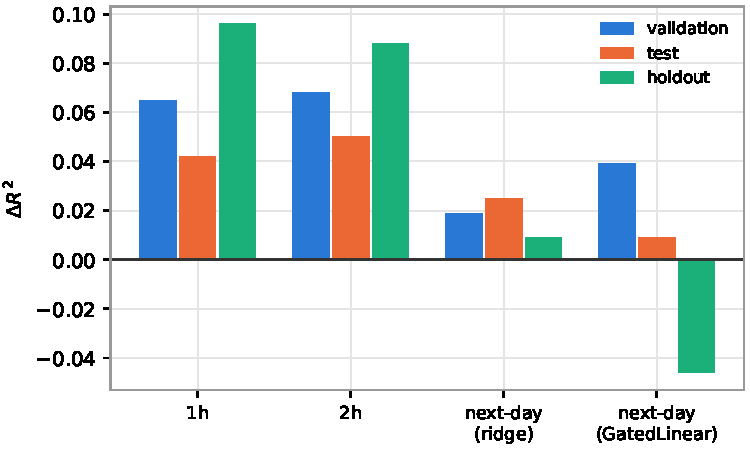
\includegraphics[width=.72\linewidth]{fig_term}
\caption{\textbf{Term structure of the hidden-state increment.} The
information horizon is strictly intraday. The daily-frequency gated corrector
illustrates validation-selected overfitting that only the pre-registered
holdout exposes.}
\label{fig:term}
\end{figure}


\begin{figure}[t]
\centering
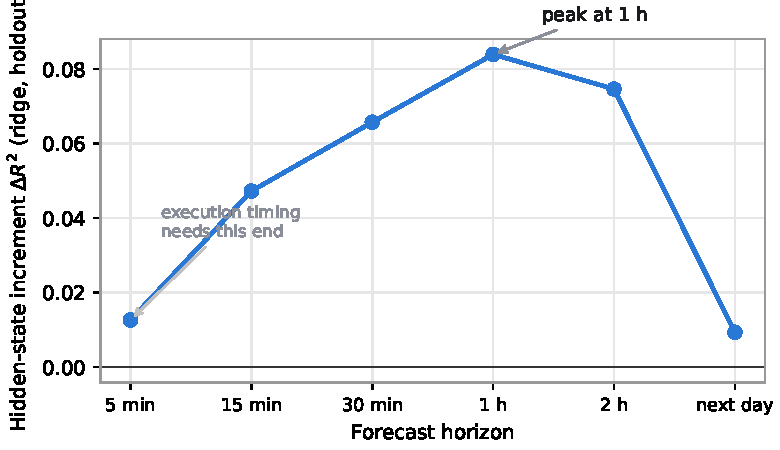
\includegraphics[width=.66\linewidth]{fig_horizon}
\caption{\textbf{The hidden-state increment has a characteristic timescale.}
Incremental $R^2$ from adding the frozen model's hidden state to the baseline,
by forecast horizon, on the pre-registered holdout (ridge specification, so all
horizons are compared under an identical estimator). The profile peaks at one
hour. Execution scheduling requires accuracy at the left end, where the
increment is smallest---which is why it fails (Section~\ref{sec:econ}).}
\label{fig:horizon}
\end{figure}

\textbf{Tails: symmetric only.} The 95th percentile of future absolute returns
inherits the full gain ($+0.033$--$0.070$); signed value-at-risk pinball
losses improve by only $\pm2$--$6\%$ with mixed signs, and crash-probability
AUC moves by $\pm0.01$.

\textbf{Subsumption of cross-sectional breadth.} Against a panel of four
cross-sectional signals built from all 500 index constituents (breadth
entropy, breadth NLL, close-location and upper-wick breadth), the hidden-state
increment is undiminished ($+0.053$--$0.058$), while the breadth increment
conditional on the hidden state is $+0.001$: one index series passed through a
frozen TSFM contains the volatility-relevant content of the 500-stock
cross-section.

%---------------- 6 Pretraining necessity ----------------
\section{Is Pretraining Necessary?}\label{sec:pretraining}
\subsection{Scratch networks and data efficiency}
A scratch Transformer (dimension 64, two layers) trained end-to-end on the
identical normalized window---without the model-derived scalars---matches the
frozen pipeline on validation and holdout at full sample size
($+0.065/+0.035/+0.096$), trailing only on the test segment; a scratch GRU and
a PCA-512 control fall short everywhere. The decisive comparison is data
efficiency (Figure~\ref{fig:dataeff}): restricted to the most recent 50\% of
training days (about 4.5 years), the frozen representation retains $+0.074$
on the holdout (77\% of its full-sample gain) versus $+0.033$ (34\%) for the
scratch model; at 15\% the ordering is the same; at 5\% both fail, with the
high-dimensional corrector failing worse. The premium of the pretrained
representation is concentrated precisely in the data regime practitioners
occupy.

\begin{figure}[t]
\centering
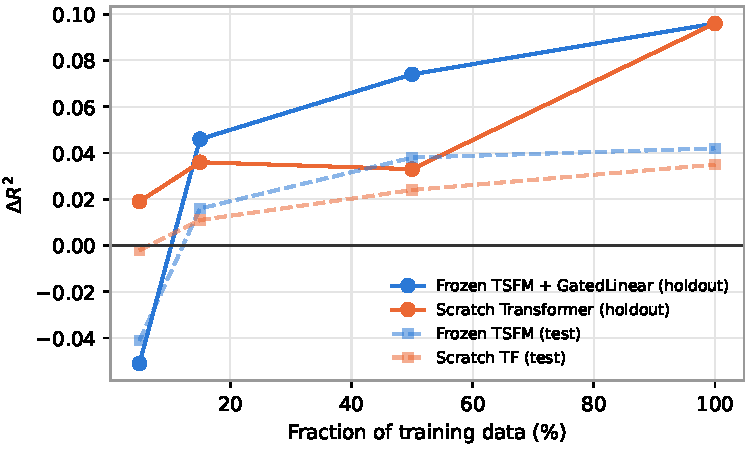
\includegraphics[width=.72\linewidth]{fig_dataeff}
\caption{\textbf{Data efficiency: the economic case for pretraining.}
Incremental $R^2$ as a function of the fraction of training data (most recent
days retained; both arms share the correspondingly re-fit baseline). The
frozen representation reaches most of its full-sample gain with half the
data; the scratch Transformer requires all of it.}
\label{fig:dataeff}
\end{figure}


\subsection{Representation scale, model class, and extraction views}
Kronos-base (four times the parameters) adds only $+0.002$--$0.008$ by ridge;
the small model saturates this task. A univariate Chronos-T5-small encoder on
close prices alone yields a real but three-times-smaller increment ($+0.056$
on holdout by ridge): the phenomenon is generic to TSFMs, while multivariate
OHLCV input and K-line-domain pretraining explain Kronos's advantage.
Multi-layer and multi-position extraction (four concatenated views, 2{,}048
dimensions) markedly improves the \emph{linear} interface (test
$+0.034 \to +0.051$) but does not surpass the production single-view gated
corrector: the nonlinear corrector already performs the cross-position
aggregation internally.

\subsection{Transfer}
Within the broad-cap family, a corrector trained on CSI~300 and CSI~1000 only
transfers to CSI~500 at full strength ($+0.055/+0.063/+0.102$). Zero-shot
transfer to style indices (SSE~50, ChiNext, STAR~50) retains only
$+0.001$--$0.012$, but re-fitting the 35K-parameter corrector locally on the
frozen representation recovers $+0.023$--$0.062$: the representation is
universal; the corrector mapping is family-specific. Figure~\ref{fig:transfer} summarizes both experiments.

\begin{figure}[t]
\centering
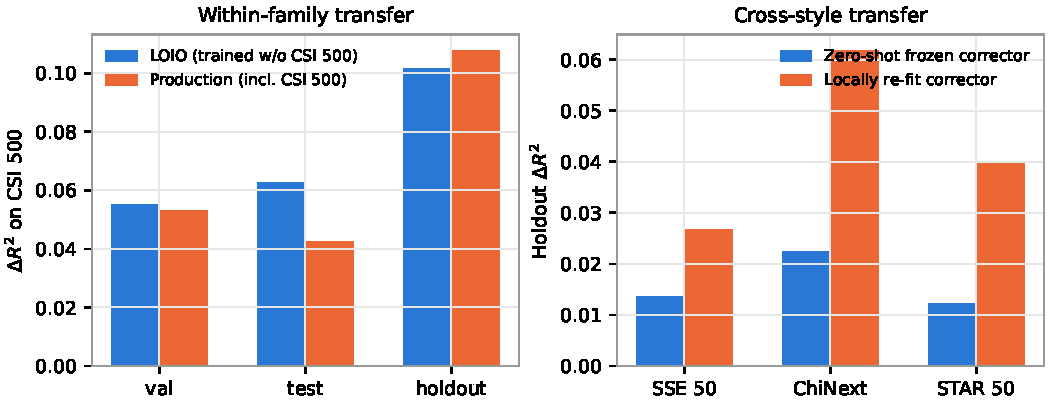
\includegraphics[width=.9\linewidth]{fig_transfer}
\caption{\textbf{Transfer of the corrector.} Left: leave-one-index-out
training within the broad-cap family transfers to CSI~500 at full strength.
Right: zero-shot transfer of the frozen corrector to style indices retains
only a fraction of the gain (holdout shown), while re-fitting the
35K-parameter corrector locally on the frozen representation restores most of
it.}
\label{fig:transfer}
\end{figure}


%---------------- 7 Economic application ----------------
\section{Economic Application: A Futures Overlay under Realistic
Costs}\label{sec:econ}
We map forecasts to positions by volatility targeting with a trend gate and a
no-trade band,
\begin{equation}
w_t = 1 + \Big[\mathrm{clip}\big(\sigma^*/\hat{\sigma}_t,\,1,\,3\big) - 1\Big]
\cdot \mathbf{1}\{\mathrm{mom}_{k,t-1} > 0\},
\qquad \sigma^* = \mathrm{median}_{\mathrm{tr}}(\hat\sigma),
\end{equation}
executing a change only when $|w_t - w^{\mathrm{cur}}| \ge \delta = 0.3$; all
hyperparameters are chosen on train-plus-validation and frozen. Daily strategy
returns follow close-to-close accounting with within-contract futures returns
$r_t$ and the asymmetric Chinese fee schedule,
\begin{equation}
R_d = \sum_{t \in d} w_{t-1} r_t
 - c^{+}(\Delta w_t)_{+} - c^{-}(\Delta w_t)_{-} - c^{\mathrm{roll}}_t ,
\qquad c^{+} = 0.55\,\mathrm{bp},\; c^{-} = 3.77\,\mathrm{bp},
\end{equation}
where intraday close-outs cost roughly seven times more than opens and
day-first reductions and rolls are charged at the overnight rate. The no-trade band cuts
daily turnover from 1.4 to 0.4 and is what keeps the overlay alive under the
close-out fee.

Replacing the baseline forecast with the hidden-state forecast in an otherwise
identical overlay is worth $+450$ to $+971$ basis points per year on IC and
$+464$ to $+690$ on IM (six of six index-segment cells positive; best cell
$t=2.3$; Figure~\ref{fig:signal}); the break-even symmetric cost is
approximately 3 basis points (Figure~\ref{fig:cost}). Table~\ref{tab:econ} summarizes the overlay economics. Against passively holding the (discounted)
futures, the gated overlay is positive in all four frozen cells
($+162$--$606$ basis points) but with $t<1.5$, and stationary-bootstrap 95\%
intervals for both comparisons include zero. We report this gap deliberately:
forecast improvements that are overwhelming by Clark--West standards can still
be marginal at the strategy level once carry, overnight gaps, and costs enter.
The deployment we endorse is an overlay for accounts that already hold a
\emph{net long} index-futures position: applying the same rule to a short
hedging leg reverses the sign of the gain (the increment comes from levering
up in low-volatility states, which coincide with positive drift), so the
overlay is not a general position-scaling device. We also note that the scaling exponent is a regime
bet: $1/\sigma^2$ scaling \citep[as in][]{moreira2017volmanaged} outperforms
in the calm holdout year and underperforms sharply in the test year, whereas
the forecast upgrade improves the $1/\sigma$ overlay in all four cells.

\begin{table}[t]
\centering\small
\caption{\textbf{Futures overlay economics.} The left block compares
volatility-targeted overlays driven by the hidden-state forecast (V2) versus
the baseline forecast (V1) in identical construction (symmetric one-basis-point
cost); annualized return differences with Newey--West $t$ statistics in
parentheses. The right block compares the frozen gated overlay (trend gate,
no-trade band, realistic asymmetric costs) with passively holding the dominant
contract. All configuration choices use train-plus-validation data only.}
\label{tab:econ}
\vspace{6pt}
\begin{tabular}{llcc@{\hspace{18pt}}cc}
\toprule
 & & \multicolumn{2}{c}{Forecast upgrade (V2$-$V1)} &
 \multicolumn{2}{c}{Overlay vs.\ buy-and-hold} \\
Product & Segment & bp/year & ($t$) & Sharpe & BH Sharpe \\
\midrule
IC & Validation & $\mathbf{+450}$ & $(1.39)$ & --- & --- \\
IC & Test & $+63$ & $(0.17)$ & $0.94$ & $0.88$ \\
IC & Holdout & $\mathbf{+971}$ & $\mathbf{(2.28)}$ & $\mathbf{1.42}$ & $1.36$ \\
IM & Validation & $\mathbf{+690}$ & $(1.81)$ & --- & --- \\
IM & Test & $+483$ & $(1.23)$ & $1.13$ & $1.15$ \\
IM & Holdout & $+464$ & $(1.00)$ & $\mathbf{1.29}$ & $1.17$ \\
\bottomrule
\end{tabular}
\end{table}


\begin{figure}[t]
\centering
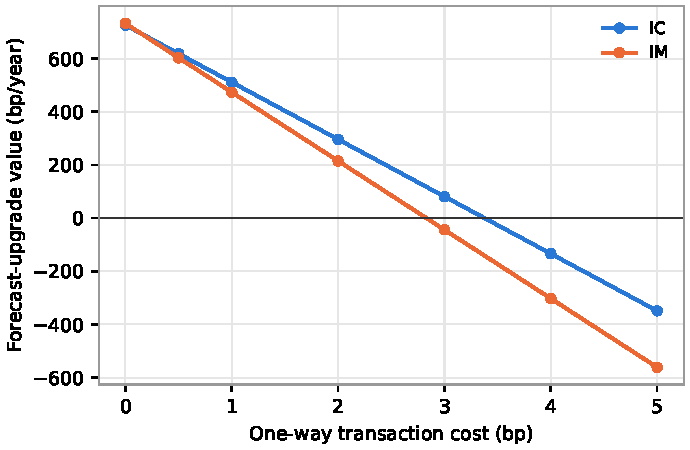
\includegraphics[width=.6\linewidth]{fig_cost}
\caption{\textbf{Cost sensitivity of the forecast upgrade.} Annualized value
of replacing the baseline forecast with the hidden-state forecast in an
identical overlay, as a function of the symmetric one-way transaction cost
(test and holdout combined). The break-even cost is approximately three basis
points for both contracts.}
\label{fig:cost}
\end{figure}


\begin{figure}[t]
\centering
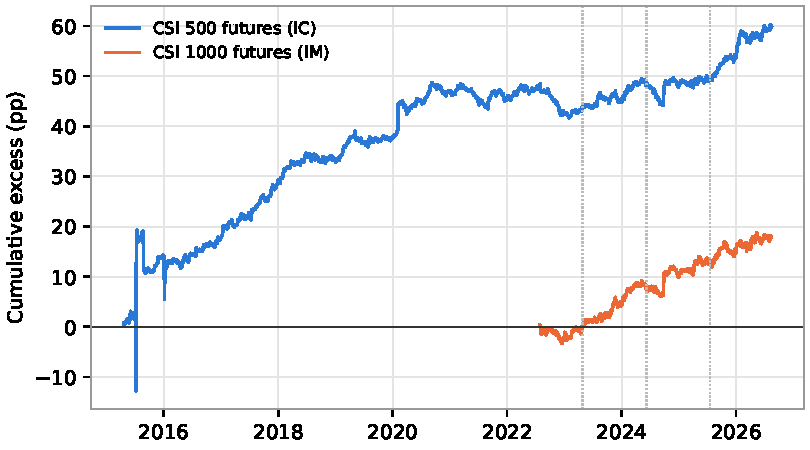
\includegraphics[width=.78\linewidth]{fig_signal}
\caption{\textbf{Cumulative value of the forecast upgrade on index futures.}
Cumulative daily return difference between volatility-targeted overlays driven
by the hidden-state forecast versus the baseline forecast (identical
construction, one-basis-point cost), with within-contract returns, overnight
gaps, and roll accounting. Dotted lines mark the validation/test/holdout
boundaries.}
\label{fig:signal}
\end{figure}


%---------------- 8 Robustness ----------------
\subsection{The position map, not the forecast, is the binding constraint}
\label{sec:mapping}
Comparing our overlay against a textbook rule driven by one-day trailing
realized volatility exposes where the forecast advantage is lost. Under the
production rule with realistic costs the two are statistically
indistinguishable, despite a holdout forecasting gap of $R^2 = 0.493$ versus
$0.634$. Two mechanisms attenuate the signal. First, \emph{truncation}: the map
$w = \mathrm{clip}(\sigma^*/\hat\sigma,1,3)$ pins 79\% of observations at unit
exposure, so most forecast variation never reaches the portfolio. Second,
\emph{turnover}: a more responsive forecast trades more, and intraday
close-outs are penalized sevenfold.

Replacing the truncating map with a smooth one confirms the diagnosis. With the
mapping family selected on train-plus-validation and frozen thereafter,
truncating maps deliver negative increments over the textbook rule in all four
frozen product-segment cells ($-276$ to $-689$\,bp per year), while
exponentially smoothed and soft-power maps deliver positive increments in all
of them ($+7$ to $+976$\,bp). Smoothing preserves the ordering of the forecast
while controlling turnover; truncation discards the ordering outright.

This is precisely the structure implied by \citet{garleanu2013dynamic}, whose
framework solves for the position path when returns are predictable and trading
is costly. Its solution takes two forms: with proportional costs the optimum is
a no-trade band---exactly the $\delta$ rule we arrived at empirically---while
with quadratic costs it is partial adjustment toward an aim portfolio,
$w_t = (1-a)w_{t-1} + a\,\mathrm{aim}_t$, which is exponential smoothing. We
estimate all inputs from the data rather than tuning them: the aim portfolio's
mean-reversion rate ($\phi = 0.0216$ per bar, a half-life of $32$ bars
$\approx 2.7$ hours, itself consistent with the one-hour peak of
Figure~\ref{fig:horizon}), the per-bar return variance, and a quadratic cost
coefficient matched to the fee schedule at the typical trade size. The
resulting trading rate,
\begin{equation}
a^{*} = \frac{\sqrt{(G+\lambda\rho)^2 + 4G\lambda} - (G+\lambda\rho)}{2\lambda}
= 0.302, \qquad G \equiv \gamma\Sigma,
\end{equation}
is obtained with \emph{zero} tuning and delivers holdout Sharpe ratios of
$2.03$ (IC) and $1.59$ (IM), matching the grid-searched smoothing constant
($2.02$ and $1.68$) while consuming no out-of-sample degrees of freedom. The
implied shrinkage of the aim portfolio, $G/(G+a^{*}\lambda\phi) = 0.95$, is
mild, as it should be for a signal whose half-life exceeds the rebalancing
interval by two orders of magnitude. That the empirically superior map is
smoothing rather than banding suggests effective costs here are dominated by
impact (quadratic) rather than fees (proportional).

\subsection{Where the forecast cannot be monetized}
The horizon curve also predicts a failure. Execution scheduling---choosing
which bars to trade a fixed quantity in, which incurs no incremental
turnover---requires accuracy at the one-bar horizon, precisely where the
hidden-state increment is smallest ($+0.013$). Under a causal participation
schedule, the baseline forecast reduces volume-weighted realized volatility by
$3.85\%$ relative to a uniform schedule and the textbook rule by $1.04\%$, but
the hidden-state forecast by only $2.97\%$: adding a horizon-mismatched signal
makes execution worse, not better. Cost-aware end-to-end training fails in both
variants we tried---restricting the loss to the interior of the position map
collapses forecast accuracy, and optimizing net profit directly halves holdout
Sharpe---because return realizations are too noisy to supervise a
35K-parameter map. At this signal-to-noise ratio, forecasting accurately and
then using the forecast rationally dominates learning the decision end to end.

\section{Robustness}\label{sec:robust}
Our conclusions survive the following checks. (i)~One hundred re-trainings
from independent seeds: holdout $\dR = +0.095\pm0.004$ with no negative seed.
(ii)~A placebo that shuffles hidden states across days within the same
intraday bar collapses the gain to the scalar level. (iii)~Annual walk-forward
refits versus frozen coefficients differ by at most $\pm0.005$ over three
years. (iv)~All sixteen cells of the overlay hyperparameter grid are positive
in both frozen segments, and the selected cell lies \emph{below} the grid
median on the holdout, so reported overlay numbers are conservative.
(v)~Every selection uses train-plus-validation data only. (vi)~A complete
no-look-ahead audit (twelve design checks and six empirical checks) accompanies
the code, including the one-day lag of the dominant-contract map and the
within-contract construction of futures returns.

\textbf{Limitations.} The forecast advantage does not translate one-for-one into
the strategy application. Under the production rule with realistic costs, a
textbook overlay driven by a one-day trailing realized volatility attains
Sharpe ratios of $0.92/1.63$ (IC) and $1.13/1.32$ (IM) on test/holdout versus
$0.94/1.41$ and $1.16/1.26$ for the hidden-state forecast---a tie, despite a
holdout forecasting gap of $R^2 = 0.493$ versus $0.634$. Two mechanisms
explain the attenuation: the position map is truncated at unit exposure for
79\% of observations, discarding most forecast variation, and the smoother
trailing estimator turns over far less under the punitive close-out fee. Our
economic claims are therefore stated strictly as V2 versus V1 (same forecast
family), and we do not claim superiority over textbook volatility targeting.
Fine-tuning (e.g., LoRA) is untested for lack of GPU
access; results concern one market and a family of related indices with
commercial minute data; the impact-cost assumption (0.32 basis points) has not
been validated against order-book data; and the corrector requires local
re-fitting outside the broad-cap index family.

%---------------- 9 Conclusion ----------------
\section{Conclusion}\label{sec:conclusion}
The unit of evaluation for foundation models in finance should be the
representation, not the model's scalar summaries. A frozen TSFM's hidden state
carries intraday second-moment information that scalar interfaces discard,
that a 500-stock cross-section does not add to, and that a scratch network can
only match with years of additional data. The practical recipe is small: one
forward pass per decision point, a 35K-parameter gated corrector, and honest
accounting on the way to the futures market.

\clearpage
\bibliographystyle{plainnat}
\bibliography{references}

%---------------- Figures and tables (at end, WP style) ----------------
\clearpage


\clearpage
\appendix
\renewcommand{\thefigure}{A\arabic{figure}}\setcounter{figure}{0}
\section*{Appendix: Additional Figures}
\noindent This appendix collects supporting robustness and mechanism figures:
the 100-seed distribution (Figure~\ref{fig:seeds}), the daily IC through time
(Figure~\ref{fig:ictime}), and the two mechanism facts
(Figures~\ref{fig:difficulty} and \ref{fig:gate}).

\begin{figure}[p]
\centering
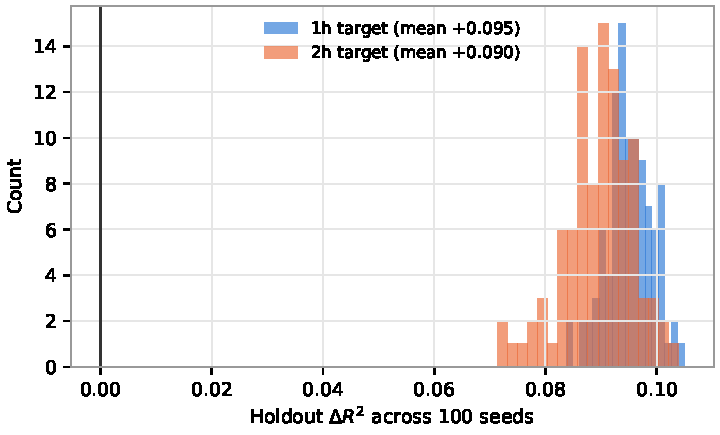
\includegraphics[width=.62\linewidth]{fig_seeds}
\caption{\textbf{Seed robustness.} Distribution of the holdout $\dR$ across
100 independent re-trainings of the gated corrector for the one-hour and
two-hour targets. No seed is negative for either target.}
\label{fig:seeds}
\end{figure}


\begin{figure}[p]
\centering
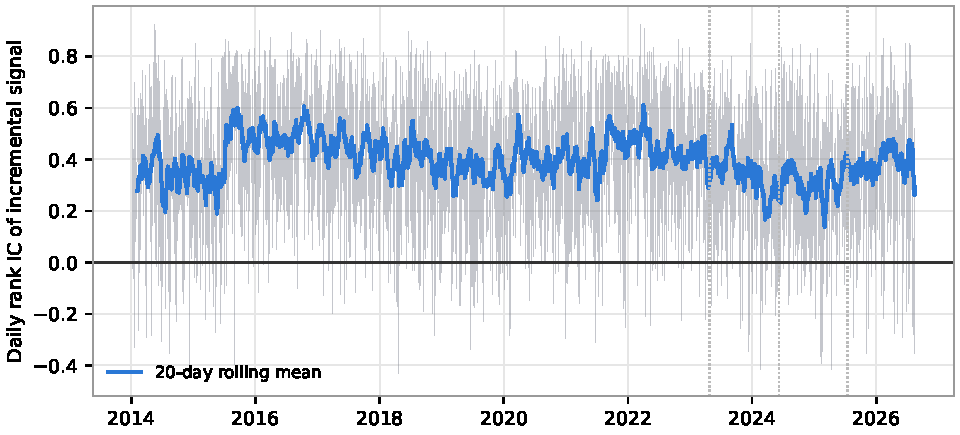
\includegraphics[width=.85\linewidth]{fig_ic_timeline}
\caption{\textbf{Daily rank IC of the incremental signal through time.} Thin
line: daily values; thick line: 20-day rolling mean. Dotted verticals mark the
validation/test/holdout boundaries. The signal does not decay out of sample: among the three out-of-sample
segments, the mean daily IC is highest in the pre-registered holdout year
(0.38 versus 0.34 and 0.31).}
\label{fig:ictime}
\end{figure}


\begin{figure}[p]
\centering
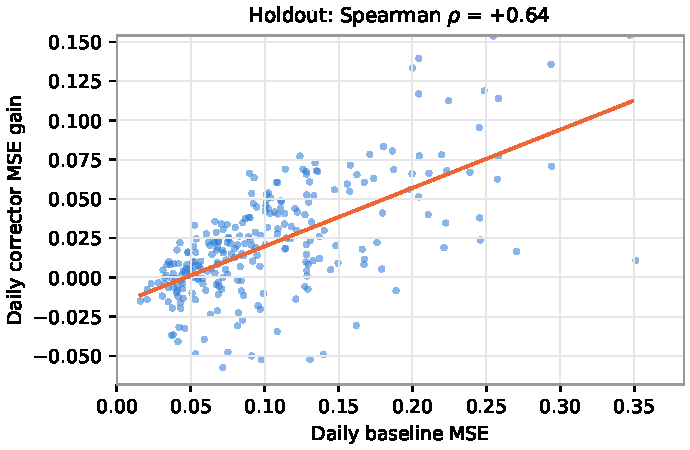
\includegraphics[width=.6\linewidth]{fig_difficulty}
\caption{\textbf{Gains concentrate where the baseline fails.} Each dot is one
holdout day: daily baseline mean-squared error against the corrector's daily
MSE gain, with an OLS fit. The Spearman correlation is $+0.64$ on the holdout
($+0.57$ and $+0.55$ on validation and test).}
\label{fig:difficulty}
\end{figure}


\begin{figure}[p]
\centering
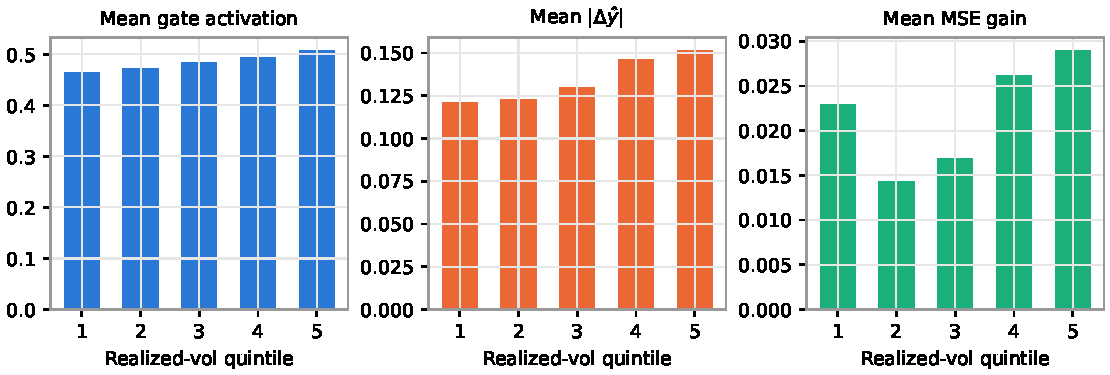
\includegraphics[width=.95\linewidth]{fig_gate}
\caption{\textbf{The learned gate opens with volatility.} Holdout means of the
gate activation $\sigma(W_g\mathbf{x})$, the absolute correction
$|\Delta\hat{y}|$, and the realized MSE gain, by train-sample
realized-volatility quintile.}
\label{fig:gate}
\end{figure}


\end{document}
